\section{Hydrodynamik: Strömungen in Flüssigkeiten}
\subsection{Stationäre Strömungen}
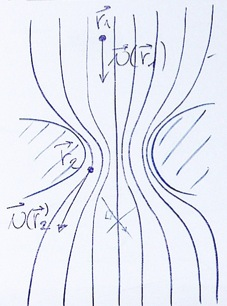
\includegraphics{Bild79} \\
Geschwindigkeitsfeld
\begin{itemize}
	\item $\vec{v}(\vec{r})$ zeitlich konst. \\
		$\rightarrow$ stationär
	\item laminare Strömung \\
		( $\bar{v} > v_{\text{krit.}} \implies$ turbulente Strömung )
\end{itemize}
\begin{def*}[ note = Volumenstromstärke (Volumendurchfluss) , index = Volumenstromstärke Volumendurchfluss , indexformat = {1 2} ]
	\[ I_V = \frac{\Delta V}{\Delta t} text{ durch Querschnitt } A \]
	Zusammenhang mit $\vec{v}$ \\
	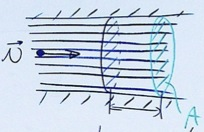
\includegraphics{Bild80} \\
	\[
		L = v \cdot \Delta t
		\intertext{in Zeit $\Delta t$}
		\Delta V = v \cdot A \cdot \Delta t \\
		\implies I_v = A \cdot v
	\]
\end{def*}

\subsection{Kontinuitätsgleichung}
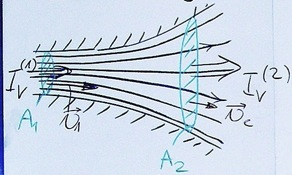
\includegraphics{Bild81}
\[
	\text{hinein: } I_V^{(1)} = A_1 \cdot v_1 \\
	\text{hinaus: } I_V^{(2)} = A_2 \cdot v_2 \\
	\implies A_1 v_1 = A_2 v_2
\]

\subsection{Die Bernoulligleichung}
Strömung unter Einfluss Druckkräften und Schwerkraft (keine Reibung!) \\
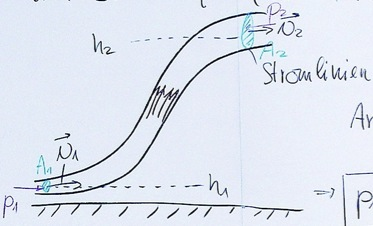
\includegraphics{Bild82} \\
Energiebilanz für Gewegung der Fl. \\
Arbeit $\Delta W$ (Druckkräfte) $- \Delta E_{\text{kin}} + \Delta E_{\text{pot}}$
\[
	\implies p_1 + \frac{1}{2} \rho v_1^2 + \rho g h_1 = p_2 + \frac{1}{2} \rho v_2^2 + \rho g h_2 \\
	\text{Gesamtdruck: } p_0 = p + \frac{1}{2} \rho v^2 + \rho g h  = \text{ statischer Druck } + \text{ dynamischer Druck } + \text{ Schweredruck}
\]

\begin{rep*}[ note = Strömungen in Flüssigkeiten ]
	Stationäre, laminare Strömungen \\
	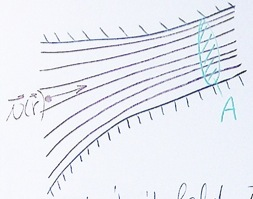
\includegraphics{Bild83} \\
	Geschwindigkeitsfeld $\vec{v}(\vec{r})$ Zeitunabhängig
	
	Volumenstromstärke:
	\[ I_v = \frac{\Delta V}{\Delta t} = A \cdot v \]
	(wenn $\vec{v}(\vec{r})$ homogen sonst:
	\[ I_v = \iint_A \vec{v} \cdot \vec{\dd A} \]
	(Fluss-Integral))
	
	Kontinuitatsgleichung \\
	\[ A_1 v_1 = A_2 v_2 \]
	
	Bernoulli-Gleichung \\
	Entlang einer reibungsfreien laminaren Strömung gilt
	\[ \underbrace*{p}_{\text{Gesamtdruck}} = \underbrace*{p_0}_{\text{stat. Druck}} + \underbrace*{\frac{1}{2} \rho v^2}_{\text{dyn. Druck}} + \underbrace*{\rho g h}_{\text{Schweredruck}} \]
	(aus Energiesatz) $h$ nach oben!
\end{rep*}

\begin{bsp*}[ note = Hydrostatik ]
	(spez. $v \equiv 0$) \\
	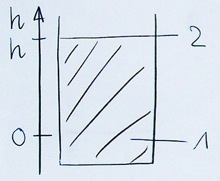
\includegraphics{Bild84} \\
	BGl.:
	\[
		p_1 + 0 + \rho g \cdot 0 = p_2 + 0 + \rho g h \\
		\implies p_1 = p_2 + \rho g h
	\]
\end{bsp*}

\subsubsection{Druckmessung in Strömungen}
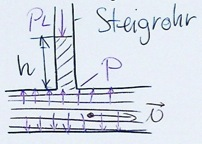
\includegraphics{Bild85}
\[ p = p_L + \rho g h \]
\begin{bsp*}[ note = Infusion ]
	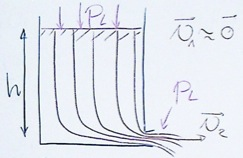
\includegraphics{Bild86} \\
	BGl.:
	\[
		\cancel{p_L} + 0 + \rho g h = \cancel{p_L} + \frac{1}{2} \rho v_2^2 + 0 \\
		\implies v_2 = \sqrt{2gh}
	\]
\end{bsp*}

\subsubsection{Mariott'sche Flasche}
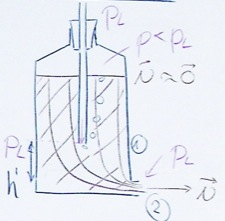
\includegraphics{Bild87}
\[ \implies v = \sqrt{2gh} = \text{ konst.} \]

\subsection{Innere Reibung}
reale Flüsigkeiten \\
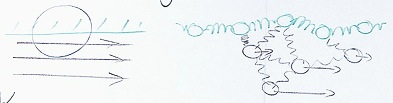
\includegraphics{Bild88} \\
Konsequenz: \\
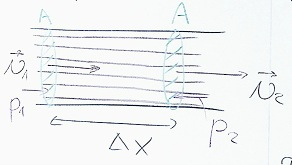
\includegraphics{Bild89} \\
Energiesatz: \\
\[
	\underbrace{\dd W}_{\text{Druckkräfte}} = \dd E_{\text{kin}} + \dd E_{\text{pot}} + \underbrace{\dd W_R}_{\text{innere Reibung}} \\
	\text{BGl: } p_1 + \frac{1}{2} \rho v_1^2 = p_2 + \frac{1}{2} \rho v_2^2 + \frac{\Delta F_R}{A}
\]
Kontinuitätsgleichung:
\[
	v_2 = v_1 \text{ !} \\
	\implies p_2 \neq p_1 ; p_2 - p_1 = \Delta p = -\frac{\Delta F_R}{A} \\
	\implies \text{ Druckabfall entlang Strömung}
\]

\subsection{Das Newtonsche Reibungsgesetz}
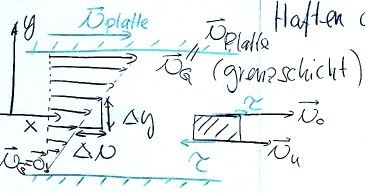
\includegraphics{Bild90} \\
Haften der Grenzschicht! \\
dynamische Schubspannung \\
Newtons Gesetz:
\[
	\tau = \eta \underbrace{\frac{\dd v}{\dd y}}_{\text{Geschwindigkeitsgefälle}} \\
	\eta \text{ Viskosität} \\
	[ \eta ] = \si{\pascal\second} \\
	1 \text{ Poise } = \SI{1}{\poise} = \SI{0.1}{\pascal\second}
\]

\subsubsection{Rohrströmungen}
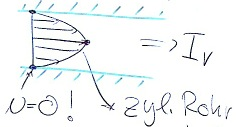
\includegraphics{Bild91} \\
$\implies$ parabolische v-Verteilung \\
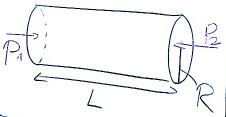
\includegraphics{Bild92}
Rechung:
\[
	v(r) = \frac{p_1 - p_2}{4 \eta L} (R^2 - r^2) \\
	\implies I_v = \iint_A \vec{v}(\vec{r}) \cdot \vec{\dd A}
\]

\subsection{Gesetz von Hagen-Poiseuille}
\[
	I_v = \frac{\pi R_4}{8 \eta L} (p_1 - p_2) \\
	I_v \sim R^4
\]
\begin{def*}[ note = Rohrwiderstand , index = Rohrwiderstand ]
	\[
		I_v = \frac{p_1 - p_2}{R_V} \\
		\implies R_V = \frac{8 \eta L}{\pi R^4}
	\]
\end{def*}

\subsubsection{Rohrsysteme}
\begin{bsp*}[ note = 2 Rohrstücke ]
	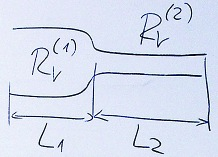
\includegraphics{Bild93} \\
	Serieschaltung
	\[ \implies R_V^{\text{Gesamt}} = R_V^{(1)} + R_V^{(2)} \]
	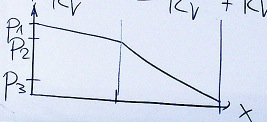
\includegraphics{Bild94}
\end{bsp*}

\begin{rep*}[ note = Hydrodynamik ]
	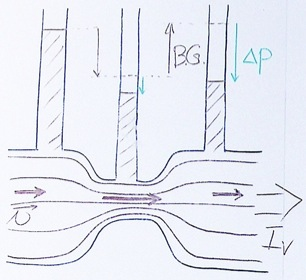
\includegraphics{Bild95} \\
	Innere Reibung $\implies$ Druckabfall $\Delta p$ entlang Strömung
	
	Newtonsches Reibungsgesetz \\
	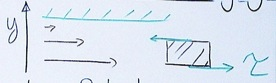
\includegraphics{Bild96} \\
	dynamische Schubspannung
	\[ \tau = \eta \frac{\dd v}{\dd y} \]
	$\eta$: Viskosität
	\[ [ \eta ] = \si{\pascal\second} \]
	
	Rohrströmungen \\
	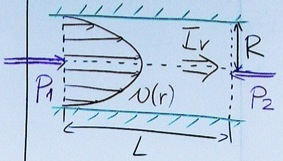
\includegraphics{Bild97}
	\[ I_v = \frac{\pi R^4}{8 \eta L} ( p_1 - p_2 ) = ( A \overline{v} ) \]
	
	Rohrwiderstand
	\[ I_v = \frac{p_1 - p_2}{R_v} \]
	( cf. $I = \frac{U}{R}$ )
	
	Gesetz von Hagen-Poiseuille \\
	Serie: \\
	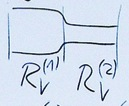
\includegraphics{Bild98}
	\[ R_v^{\text{tot}} = R_v^{(1)} + R_v^{(2)} \]
\end{rep*}

\subsubsection{Parallelschaltung}
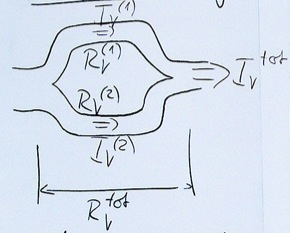
\includegraphics{Bild99}
\[ \implies \frac{1}{R_V^{\text{tot}}} = \frac{1}{R_V^{(1)}} + \frac{1}{R_V^{(2)}} \]

\subsection{Das Stokesche Reibungsgesetz}
\begin{bsp*}[ note = Kugel in Strömung ]
	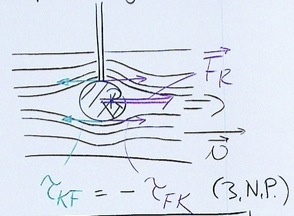
\includegraphics{Bild100}
	\[ F_R = \underbrace{6 \pi R}_{\text{Kugel}} \eta v \]
\end{bsp*}

Anwedndung: Sedimentation \\
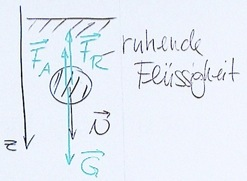
\includegraphics{Bild101} \\
2.N.P.
\[ ma = mg - m_{\text{Fl}} \cdot g - 6\pi R \cdot \eta \cdot v \]
Exp.
\[
	v = \text{ konst.} \implies a = 0 \\
	v_s = \frac{mg - m_{\text{Fl}} g}{6 \pi R \eta} \\
	v_s = \frac{\frac{4}{3} \pi R^3 (\rho_{K} - \rho_{\text{Fl}}}{6 \pi R \eta} \cdot g \\
	v_s = \frac{2}{9} \frac{( \rho_K - \rho_{\text{Fl}} )}{\eta} g R^2
\]

$\frac{\SI{50}{\milli\metre}}{\SI{30}{\minute}} \rightarrow$ Pferdeblut \\
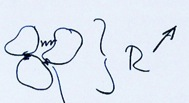
\includegraphics{Bild102} WW zwischen Blutkörperchen \\
\begin{tabular}{ l l }
	Mann: &$\SIrange{3}{7}{\milli\metre\per\hour}$ \\
	Frau: &$7 - 11 \frac{\text{mm}}{\text{h}}$ \\
	Baby: &$1 - 2 \frac{\text{mm}}{\text{h}}$
\end{tabular}

\subsection{Turbulente Stömungen}
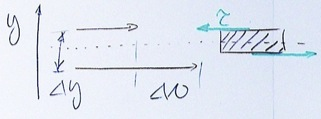
\includegraphics{Bild103} \\
$\frac{\Delta v}{\Delta y}$ grösser $\implies$ \\
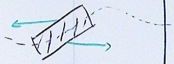
\includegraphics{Bild104} \\
Wirbelbildung

\subsubsection{Rohrströmung}
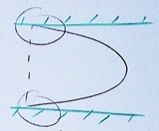
\includegraphics{Bild105} \\
$\frac{\Delta v}{\Delta y}$ gross \\
Ab wann Turbulenz? \\
Reynoldsche Zahl $Re$
\[ Re = \frac{2R\rho}{\eta} \cdot \underbrace{\overline{v}}_{\text{mittlere Strömungsgeschwindigkeit}} \]

\subsubsection{Turbulenzkriterium}
\[ Re \gtrsim \underbrace{2300}_{\text{zyl. Röhre}} \]
kritische Geschwindigkeit $v_{\text{krit}}$
\[ Re = \frac{2R\rho}{\eta} \underbrace{\overline{v}}_{v_{\text{krit}}} = 2300 \]

\begin{bsp*}[ note = Blutströmung ]
	mittlere Strömungsgeschwindigkeit $\overline{v}$
	\[
		\text{H.P: } I_V = \frac{\pi R^4}{8 \eta L} \Delta p = A \overline{v} = \pi R^2 \overline{v} \\
		\overline{v} = \frac{R^2}{8 \pi L} \Delta p
	\]
	Blut: $\rho = 10^3 \frac{\text{kg}}{\text{m}^3} ; \eta \approx 4 \cdot 10^{-3} \text{Pa} \cdot \text{s}$ \\
	Aorta:
	\[
		\left. \begin{matrix*}[l]
			R &\approx 1 \cdot 10^{-2} \text{m} \\
			L &\approx 0.4 \text{m} \\
			\Delta p &\approx 40 \text{Pa}
		\end{matrix*} \right\} \begin{matrix*}[l]
			\overline{v} = 0.3 \frac{\text{m}}{\text{s}} \\
			Re = 1500
		\end{matrix*} \implies
	\]
	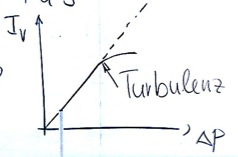
\includegraphics{Bild106}
\end{bsp*}

\subsubsection{Kapillare}
\[
	\left. \begin{matrix*}[l]
		R &\approx 4 \cdot 10^{-6} \text{m} \\
		L &\approx 0.001 \text{m} \\
		\Delta p &\approx 10^3 \text{Pa}
	\end{matrix*} \right\} \begin{matrix*}[l]
		\overline{v} = 5 \cdot 10^{-4} \frac{\text{m}}{\text{s}} \\
		Re = 0.001
	\end{matrix*} \implies \text{ nie Turbulent}
\]

\begin{rep*}[ note = Hydrodynamik ]
	Das Stoke'sche Reibungsgesetz \\
	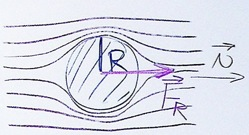
\includegraphics{Bild107}
	\[ F_R = 6 \pi R \eta v \]
	
	Turbulente Strömung \\
	Reynoldszahl $Re = \frac{2R \cdot \rho}{\eta} \overline{v}$ \\
	Turbulenzkriterium: $\overline{v} \gtrsim v_{\text{krit}}$ \\
	Rohrströmung: $Re \gtrsim 2300$
\end{rep*}
